\documentclass[UTF8,titlepage]{ctexart}
\usepackage{amsmath,amssymb,amsthm,amsfonts,amscd}
\usepackage{fontspec}
\setmainfont{Times New Roman}
\usepackage{graphicx}
\usepackage{titlesec}
\usepackage{makecell}
\usepackage{longtable}
\usepackage{xcolor}
\usepackage{tcolorbox}
\usepackage{soul}
\usepackage{adjustbox}
\usepackage{tcolorbox}
\usepackage{enumerate}
\usepackage{pdfpages}
\usepackage{float}
\usepackage{colortbl}
\usepackage{tabularx}
\usepackage{multirow}
\usepackage{pgfplots}
\usepackage[utf8]{inputenc}
\usepackage{booktabs}
% \usepackage{algorithm}
% \usepackage{algorithmic}
<<<<<<< HEAD
\usepackage{algpseudocode}
\usepackage[utf8]{inputenc}
\usepackage[ruled,vlined]{algorithm2e}

=======
% \usepackage{algpseudocode}
\usepackage[linesnumbered,ruled,vlined]{algorithm2e}
% \SetKwBlock{Begin}{begin}{end} % 添加这一行来定义 Begin-End
>>>>>>> ec0ee5f926962128ee0f5c971782087db85c92d8
\numberwithin{figure}{section}
\usepackage[left=1.25in,right=1.25in,%
top=1in,bottom=1in]{geometry}
\usepackage{color}
\titleformat{\section}
  {\raggedright\LARGE\bfseries}{\thesection}{1em}{}
\begin{document}
\title{算法导论课程报告 \\ \large{——01背包问题的求解与分析}}
\author{赵伯远 \\ 211440128}
\date{\today}
\maketitle

\tableofcontents


\clearpage

\section{问题描述}

01背包问题是组合优化问题中的一个经典问题,其背景可以追溯到物品的装载和资源的分配。具体来说,假设有一个背包,其承载的最大重量为\( C \)。同时,有\( n \)个物品,每个物品有各自的重量\( w_i \)和价值\( v_i \)。01背包问题的目标是选择一些物品装入背包中,使得这些物品的总重量不超过背包的最大承载重量,而它们的总价值尽可能大。

形式化地,可以将问题描述如下:

\textbf{目标:}
\begin{equation}
    \max \sum_{i=1}^{n} v_i \cdot x_i
\end{equation}

\textbf{受到约束:}
\begin{equation}
    \sum_{i=1}^{n} w_i \cdot x_i \leq C
\end{equation}

\textbf{其中:}
\begin{itemize}
    \item \( x_i \) 是一个二元变量,如果物品\( i \)被选中,则\( x_i = 1 \);如果没有被选中,则\( x_i = 0 \)。
    \item \( v_i \) 是物品\( i \)的价值。
    \item \( w_i \) 是物品\( i \)的重量。
    \item \( C \) 是背包的最大承重。
\end{itemize}

\section{算法分析}

\subsection{蛮力法}

\subsubsection{朴素方法}

朴素的蛮力法的核心思想是检查所有可能的物品组合。对于每种组合,我们计算其总重量和总价值,并检查总重量是否超过背包的最大容量。如果没有超过,我们将其与当前找到的最大价值进行比较,以更新最大价值。

\begin{algorithm}[H]
    \SetAlgoLined
    \DontPrintSemicolon
<<<<<<< HEAD
    \KwIn{$weights$ -- list of item weights, $values$ -- list of item values, $capacity$ -- knapsack capacity}
=======
    \KwIn{$weights$, $values$ , $capacity$ }
>>>>>>> ec0ee5f926962128ee0f5c971782087db85c92d8
    \KwOut{Maximum value achievable}
    \caption{BruteForceKnapsack}
    \SetKwFunction{FBFK}{BruteForceKnapsack}
    \SetKwProg{Fn}{Function}{:}{}
    \Fn{\FBFK{$weights, values, capacity$}}{
        $maxValue \gets 0$\;
        \ForEach{$combination$}{
            \If{$Weight(combination) \leq capacity$}{
                $maxValue \gets \max(maxValue, Value(combination))$\;
            }
        }
        \KwRet $maxValue$\;
    }
    \end{algorithm}

\subsubsection{位运算优化}
位运算优化方法是朴素方法的一种改进。在这种方法中,我们使用整数的二进制表示来表示物品的选择状态。每个位代表一个物品,其中 1 表示选择该物品,0 表示不选择。

通过遍历从 0 到 $2^n - 1$ 的所有整数,我们可以有效地遍历所有物品的组合。对于每个整数,我们使用位运算来确定哪些物品被选中,并计算这些物品的总重量和总价值。这种方法在理论上与朴素方法相同,但在实践中通常更高效,因为它直接利用了计算机的二进制运算能力(常数优化)。

\begin{algorithm}[H]
    \SetAlgoLined
    \DontPrintSemicolon
    \KwIn{$weights$, $values$ , $capacity$ }
    \KwOut{Maximum value achievable}
    \caption{BitwiseOptimizedKnapsack}
    \SetKwFunction{FBOK}{BitwiseOptimizedKnapsack}
    \SetKwProg{Fn}{Function}{:}{}
    \Fn{\FBOK{$weights, values, capacity$}}{
        $maxValue \gets 0$\;
        \For{$i \gets 0$ \KwTo $2^n - 1$}{
            $weight \gets 0, value \gets 0$\;
            \For{$j \gets 0$ \KwTo $n - 1$}{
                \If{$i$ \& $(1 \ll j)$}{
                    $weight \gets weight + weights[j]$\;
                    $value \gets value + values[j]$\;
                }
            }
            \If{$weight \leq capacity$}{
                $maxValue \gets \max(maxValue, value)$\;
            }
        }
        \KwRet $maxValue$\;
    }
    \end{algorithm}

\subsection{动态规划}

\subsubsection{朴素方法}

在二维数组方法中,我们定义 $dp[i][v]$ 为用剩余容量为 $v$ 的背包来装前 $i$ 件物品时可以达到的最大价值。因此,状态转移方程如下:

\[ dp[i][0] = 0 \]

对于每个物品 $i$ 和每个可能的容量 $v$,有以下两种情况:

\begin{itemize}
  \item 如果物品 $i$ 的体积大于 $v$,即 $w[i] > v$,则当前物品无法装入背包,所以 $dp[i][v] = dp[i-1][v]$。
  \item 如果物品 $i$ 的体积不大于 $v$,即 $w[i] \leq v$,则有两种选择:装入物品 $i$ 或者不装入。因此,状态转移方程为:
  \[ dp[i][v] = \max(dp[i-1][v], dp[i-1][v-w[i]] + p[i]) \]
\end{itemize}

在这里,$w[i]$ 和 $p[i]$ 分别代表物品 $i$ 的重量和价值。

\begin{algorithm}[H]
\SetAlgoLined
\DontPrintSemicolon
\KwIn{$weights$, $values$ , $capacity$ }
\KwOut{Maximum value achievable}
\caption{TwoDimensionalKnapsack}
\SetKwFunction{FBDP}{TwoDimensionalKnapsack}
\SetKwProg{Fn}{Function}{:}{}
\Fn{\FBDP{$weights, values, capacity$}}{
    $dp \gets$ array[0..length($weights$)][0..$capacity$] initialized to 0\;
    \For{$i \gets 1$ \KwTo length($weights$)}{
        \For{$w \gets 0$ \KwTo $capacity$}{
            \uIf{$weights[i] \leq w$}{
                $dp[i][w] \gets \max(dp[i-1][w], dp[i-1][w-weights[i]] + values[i])$\;
            }
            \Else{
                $dp[i][w] \gets dp[i-1][w]$\;
            }
        }
    }
    \KwRet $dp[$length($weights$)$][$capacity$]$\;
}
\end{algorithm}

\subsubsection{滚动数组优化}
在标准的二维数组方法中,我们使用一个二维数组 $dp[i][w]$ 来存储所有可能的状态。然而,实际上,在计算 $dp[i][w]$ 时,我们只需要前一行 $i-1$ 的数据。这意味着,我们并不需要存储整个二维数组来获得最终结果,而只需保留足够的信息来推导出当前行的值。

滚动数组的优化基于这样一个观察:在计算第 $i$ 行的状态时,只需要第 $i-1$ 行的状态。因此,我们可以使用两个一维数组交替表示当前行和上一行,而不是使用完整的二维数组。这种方法大大减少了空间复杂度,从 \(O(nC)\) 减少到 \(O(2C)\),其中 \(n\) 是物品的数量,\(C\) 是背包的容量。我们通过交替更新两个数组,以保持动态规划的正确性,同时节约空间。

状态转移方程改写如下:
\begin{equation}
    dp[current][w] = \max(dp[previous][w], dp[previous][w-weights[i]] + values[i])
\end{equation}

这里,$current$ 和 $previous$ 分别代表当前和前一行的索引。这种方法通过交替使用两个数组(或两行),减少了空间的需求,同时保持了动态规划的核心逻辑不变。

\begin{algorithm}[H]
    \SetAlgoLined
    \DontPrintSemicolon
    \KwIn{$weights, values, capacity$}
    \KwOut{Maximum value achievable}
    \caption{RollingArrayKnapsack}
    \SetKwFunction{FBRA}{RollingArrayKnapsack}
    \SetKwProg{Fn}{Function}{:}{}
    \Fn{\FBRA{$weights, values, capacity$}}{
        $dp \gets$ array[2][0..$capacity$] initialized to 0\;
        \For{$i \gets 1$ \KwTo length($weights$)}{
            \For{$w \gets 0$ \KwTo $capacity$}{
                \uIf{$weights[i-1] \leq w$}{
                    $dp[i\%2][w] \gets \max(dp[(i-1)\%2][w], dp[(i-1)\%2][w-weights[i-1]] + values[i-1])$\;
                }
                \Else{
                    $dp[i\%2][w] \gets dp[(i-1)\%2][w]$\;
                }
            }
        }
        \KwRet $dp[length($weights$)\%2][$capacity$]$\;
    }
    \end{algorithm}

\subsubsection{一维数组优化}
在进一步优化,我们只使用一个一维数组 $dp[w]$。在这种情况下,更新 $dp[w]$ 时需要确保引用的 $dp[w-weights[i]]$ 是上一个物品状态的值,而非当前物品已经更新过的值。

为了确保这一点,我们采用逆序枚举的方式更新数组。这意味着对于每个物品 $i$,我们从背包的最大容量开始向下遍历到该物品的重量。逆序更新确保在更新 $dp[w]$ 时,$dp[w-weights[i]]$ 仍然代表不包含当前物品 $i$ 的情况。如果我们采用正序枚举,那么在更新 $dp[w]$ 时,$dp[w-weights[i]]$ 可能已经被当前物品更新,从而导致错误的结果。

通过逆序枚举,我们可以保证每次更新 $dp[w]$ 时,所依赖的历史数据(较小的 $w$ 值)是有效的,从而确保算法的正确性。这种方法的空间复杂度是 \(O(C)\),在实际应用中非常有效,特别是对于背包容量大但可用内存有限的情况。

状态转移方程改写如下:
\begin{equation}
    dp[w] = \max(dp[w], dp[w-weights[i]] + values[i])
\end{equation}

在这个方程中,只使用 $dp[w]$ 来存储每个容量下的最大价值。逆序更新是关键,它保证了在更新 $dp[w]$ 时,$dp[w-weights[i]]$ 仍然代表不包含当前物品 $i$ 的情况。

\begin{algorithm}[H]
    \SetAlgoLined
    \DontPrintSemicolon
    \KwIn{$weights$, $values$ , $capacity$ }
    \KwOut{Maximum value achievable}
    \caption{OneDimensionalKnapsack}
    \SetKwFunction{FBOD}{OneDimensionalKnapsack}
    \SetKwProg{Fn}{Function}{:}{}
    \Fn{\FBOD{$weights, values, capacity$}}{
        $dp \gets$ array[0..$capacity$] initialized to 0\;
        \For{$i \gets 0$ \KwTo length($weights$) - 1}{
            \For{$w \gets capacity$ \KwTo $weights[i]$ \textbf{step} -1}{
                $dp[w] \gets \max(dp[w], dp[w - weights[i]] + values[i])$\;
            }
        }
        \KwRet $dp[capacity]$\;
    }
    \end{algorithm}


\subsection{遗传算法}

\subsubsection{遗传算法简介}
遗传算法是一种模仿自然界生物进化机制的优化方法,通过迭代过程在解空间中搜索最优解。对于01背包问题,我们可以利用遗传算法高效地探索潜在的最优解。

首先,算法随机初始化一个种群,每个个体由一系列基因组成,这些基因代表背包中物品的装载状态,即1代表装入,0代表不装入。种群的每个个体都是一个潜在的解决方案。

适应度函数是遗传算法的核心,用于评价个体的适应程度。对于01背包问题,适应度函数通常是个体中所选物品的总价值,但需要注意的是,若个体所选物品的总重量超过背包容量,则应对该个体进行惩罚,使其适应度为0。这样可以确保选出的解是有效的。

在每一代中,算法首先根据适应度对种群进行排序,以确保更适应的个体有更高的存活概率。然后,算法通过交叉和变异操作产生新的个体。交叉操作模仿生物的繁殖过程,从两个父本个体中创造出新的后代,而变异操作则随机改变个体的某些基因,增加种群的多样性。

通过重复这个过程,种群逐渐进化,适应度较高的个体逐渐占据主导地位。最终,算法通过选择适应度最高的个体作为问题的最优解。这个过程不断迭代,直到满足特定的停止条件,如达到预设的代数。

    
\subsubsection{锦标赛选择}

由于基础的遗传算法表现不佳,因此我们可以考虑引入更加优秀的选择算子。锦标赛选择是一种常用的选择算子,用于从种群中选择个体。在锦标赛选择中,我们随机选择 $k$ 个个体,然后从中选择适应度最高的个体作为父本。这个过程重复 $n$ 次,直到选择出 $n$ 个父本。

\begin{algorithm}[H]
    \SetAlgoLined
    \DontPrintSemicolon
    \caption{Knapsack Genetic Algorithm with Tournament Selection}
    \KwIn{Items, C, PopulationSize, Generations, CrossoverRate, MutationRate, TournamentSize}
    \KwOut{Maximum value achieved by the knapsack}
    
     Initialize random number generator\;
     Initialize population with random individuals\;
     \ForEach{individual in population}{
      \ForEach{gene in individual}{
       gene = random value (0 or 1)\;
      }
     }
    
     Define fitness function\;
     
     \For{generation = 0 to Generations}{
      Initialize newPopulation\;
      \For{i = 0 to PopulationSize}{
       Select parent1 and parent2 using tournament selection\;
       Initialize child\;
       \uIf{random number < CrossoverRate}{
        Perform crossover between parent1 and parent2\;
       }
       \Else{
        child = parent1\;
       }
       \ForEach{gene in child}{
        \If{random number < MutationRate}{
         Mutate gene\;
        }
       }
       Add child to newPopulation\;
      }
      Replace population with newPopulation\;
      Sort population based on fitness\;
      Update answer with the fitness of the best individual\;
     }
     Sort population based on fitness\;
     \KwRet{Maximum fitness value}\;
    \end{algorithm}
\clearpage

\subsection{算法效率分析}

在01背包问题中,不同的算法有各自的优势和限制。以下是一些主要算法的时间和空间复杂度的分析。

\subsection{蛮力法}
蛮力法通过枚举所有可能的物品组合来寻找最优解。对于每个物品,有两种可能的状态(选中或未选中),因此对于 $n$ 个物品,总共有 $2^n$ 种可能的组合。因此,蛮力法的时间复杂度为 $O(2^n)$。每个组合需要 $O(n)$ 的空间来存储,因此空间复杂度为 $O(n)$。

\subsection{动态规划}
动态规划通过构建一个二维数组来避免重复计算,数组的大小为物品数量 $n$ 乘以背包容量 $C$。因此,时间和空间复杂度均为 $O(nC)$。通过优化方法如滚动数组和一维数组,可以将空间复杂度降低到 $O(2C)$ 和 $O(C)$,分别适用于空间受限和高度空间受限的情况。

\subsection{遗传算法}
遗传算法的时间复杂度取决于种群大小 $p$、代数 $g$ 和每代中的操作数量 $m$,因此时间复杂度为 $O(g \cdot p \cdot m)$。空间复杂度主要受种群大小 $p$ 影响,因此为 $O(p)$。遗传算法适用于大规模和复杂的问题,特别是在解空间较大时。
\begin{table}[htbp]
    \centering
    \caption{蛮力法、动态规划和遗传算法在01背包问题中的性能对比}
    \begin{tabular}{@{}llll@{}}
    \toprule
    算法类型 & 时间复杂度 & 空间复杂度 & 适用场景 \\ \midrule
    蛮力法 & $O(2^n)$ & $O(n)$ & 小规模问题 \\
    动态规划(朴素方法) & $O(nC)$ & $O(nC)$ & 通用 \\
    动态规划(滚动数组优化) & $O(nC)$ & $O(2C)$ & 空间受限 \\
    动态规划(一维数组优化) & $O(nC)$ & $O(C)$ & 空间高度受限 \\
    遗传算法 & $O(g \cdot p \cdot m)$ & $O(p)$ & 大规模、复杂问题 \\ \bottomrule
    \end{tabular}
    \end{table}

\newpage

\section{实验结果分析}

\subsection{实验环境}
实验环境为Github Codespaces,操作系统为Ubuntu 22.04,CPU为AMD EPYC 7763的4核心,内存为16GB。编译器为g++ 13.2.0,编译选项为-O3,C++标准为C++20。

\subsection{测试样例}
在实验中中使用了三组测试数据,分别为小规模、中等规模和大规模。小规模测试数据包含4个物品,背包容量为 ,中等规模测试数据包含8个物品,大规模测试数据包含50个物品。每个物品的重量和价值均为随机生成的正整数。

\subsection{实验结果}

\begin{figure}[H]
\centering
 \resizebox{0.75\textwidth}{!}{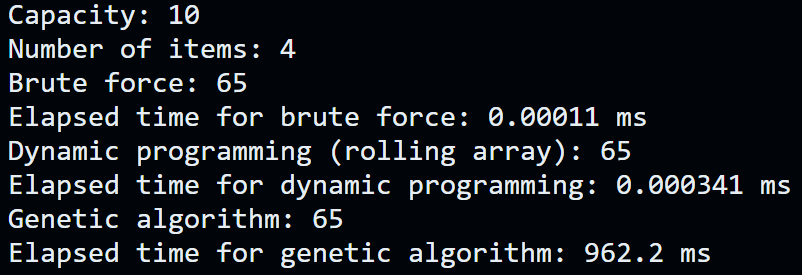
\includegraphics{./Test1.png}}
 \caption{Capacity = 10, n = 4}
 \label{}
\end{figure}

\begin{figure}[H]
\centering
 \resizebox{0.75\textwidth}{!}{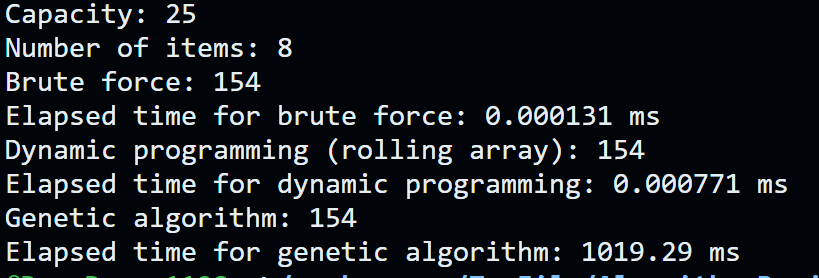
\includegraphics{./Test2.png}}
 \caption{Capacity = 25, n = 8}
 \label{}
\end{figure}

\begin{figure}[H]
\centering
 \resizebox{0.75\textwidth}{!}{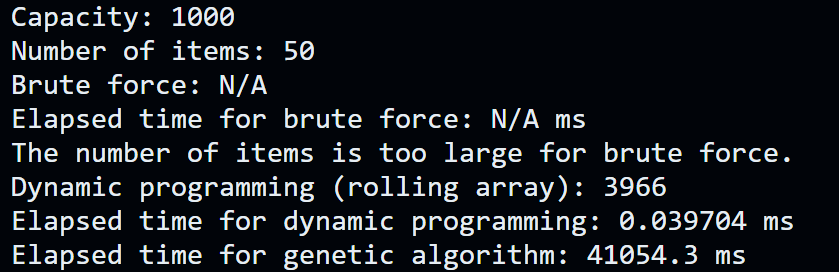
\includegraphics{./Test3.png}}
 \caption{Capacity = 100, n = 50}
 \label{}
\end{figure}

\section{总结}

\subsection*{蛮力法 (Brute Force)}

\textbf{优点:}
\begin{enumerate}
    \item 简单直观:直接枚举所有可能的物品组合,容易理解和实现。
    \item 完备性:保证可以找到最优解,因为它检查了所有可能的组合。
\end{enumerate}

\textbf{缺点:}
\begin{enumerate}
    \item 时间复杂度高:时间复杂度为 $O(2^n)$,在物品数量多的情况下非常低效。
    \item 不实用:在实际应用中几乎不可行,因为随着物品数量的增加,所需的计算时间呈指数级增长。
\end{enumerate}

\subsection*{动态规划 (Dynamic Programming)}

\textbf{优点:}
\begin{enumerate}
    \item 效率高:时间复杂度为 $O(nC)$,其中 $n$ 是物品数量,$C$ 是背包容量,比蛮力法高效得多。
    \item 确保找到最优解:动态规划通过逐步构建解决方案,确保了找到全局最优解。
    \item 空间优化:使用滚动数组可以将空间复杂度从 $O(nC)$ 优化到 $O(C)$。
\end{enumerate}

\textbf{缺点:}
\begin{enumerate}
    \item 复杂度:时间复杂度与背包容量 $C$ 线性相关,当 $C$ 很大时,仍然可能较慢。
    \item 不适用于分数或非线性问题:只适用于背包容量和物品重量都是整数的情况。
\end{enumerate}

\subsection*{遗传算法 (Genetic Algorithm)}

\textbf{优点:}
\begin{enumerate}
    \item 适应性强:适用于复杂的、非线性的和多约束的优化问题。
    \item 全局搜索能力:遗传算法通过模拟自然选择的过程,能有效地在搜索空间中进行全局搜索。
    \item 并行处理能力:可以在多个解上并行运行,适合并行处理。
\end{enumerate}

\textbf{缺点:}
\begin{enumerate}
    \item 找到的是近似解:遗传算法通常找到的是问题的近似最优解,而不是确切的最优解。
    \item 参数依赖性:算法的性能在很大程度上依赖于交叉率、变异率等参数的选择。
    \item 收敛性:可能会过早地收敛到局部最优解,而不是全局最优解。
\end{enumerate}

\subsection*{总结}

蛮力法因其低效性而很少在实际应用中使用。动态规划是解决0-1背包问题最常用的方法,它能够确保找到最优解并且在计算上更为高效。然而,当背包容量很大时,动态规划的性能也会受到影响。遗传算法是一种更灵活的搜索方法,特别适用于那些对动态规划来说过于复杂或者背包容量过大的问题。它通过模拟自然选择过程,通常能够找到问题的近似最优解,并且适合并行计算。然而,遗传算法需要仔细选择参数,并且可能需要更多的时间来逼近最优解。在选择算法时,应考虑问题的大小、背包容量、解的精确度要求以及可用计算资源等因素。





\end{document}